\section{Resoconto attività di verifica}
In questa sezione sono descritte le attività di verifica svolte sui documenti che vengono presentati alle revisioni di avanzamento. Qualora una verifica riscontrasse un problema su un documento, nella sezione \S C si discuterà di quali siano i possibili miglioramenti.
Inoltre verranno utlizzate delle sigle per stabilie il periodo in cui sono stati rilevati i risultati delle verifiche. Le sigle sono le seguenti:
\begin{itemize}
\item \textbf{An}: Analisi;
\item \textbf{TB}: Technology Baseline;
\item \textbf{PB}: Product Baseline;
\item \textbf{VC}: Validazione e Convalida. 
\end{itemize}

\subsection{Analisi dei documenti}
\subsubsection{Analisi statica} \mbox{} \\ \mbox{} \\
L'analisi dei documenti mediante Walkthrough (vedi \textit{Norme di Progetto}) ha portato all'individuazione di alcuni errori frequenti a partire dai quali è stata stilata una check list. In questo modo sarà possibile applicare l’Inspection (vedi \textit{Norme di Progetto}) per le future attività di verifica.


\paragraph{Esiti Indice di Gulpease} \mbox{} \\ \mbox{} \\
\begin{longtable}{c c c c c c}
\rowcolor{white}\caption{Esiti verifica documenti con Indice di Gulpease} \\
		\rowcolor{redafk}
\textcolor{white}{\textbf{Documento}} &
\textcolor{white}{\textbf{An}} &
\textcolor{white}{\textbf{TB}} &
\textcolor{white}{\textbf{PB}} &
\textcolor{white}{\textbf{VC}} &
\textcolor{white}{\textbf{Esito}} \\
		\endfirsthead
		\rowcolor{white}\caption[]{(continua)} \\
		\rowcolor{redafk}
\textcolor{white}{\textbf{Documento}} &
\textcolor{white}{\textbf{An}} &
\textcolor{white}{\textbf{TB}} &
\textcolor{white}{\textbf{PB}} &
\textcolor{white}{\textbf{VC}} &
\textcolor{white}{\textbf{Esito}} \\
		\endhead
		\textit{analisi\_dei\_requisiti\_v1.0.0} & 70 & - & - & - & Superato \\
		\textit{glossario\_v1.0.0} & 74 & - & - & - & Superato \\
		\textit{norme\_di\_progetto\_v1.0.0} & 67 & - & - & - & Superato \\
		\textit{piano\_di\_progetto\_v1.0.0} & 69 & - & - & - & Superato \\
		\textit{piano\_di\_qualifica\_v1.0.0} & 72 & - & - & - & Superato \\
		\textit{studio\_di\_fattibilità\_v1.0.0} & 70 & - & - & - & Superato \\
		\textit{VI\_2020-03-11} & 72 & - & - & - & Superato \\
		\textit{VI\_2020-03-18} & 76 & - & - & - & Superato \\
		\textit{VI\_2020-03-20} & 70 & - & - & - & Superato \\
		\textit{VI\_2020-03-22} & 71 & - & - & - & Superato \\
		\textit{VI\_2020-03-31} & 71 & - & - & - & Superato \\
		\textit{VE\_2020-03-16} & 70 & - & - & - & Superato \\
		\textit{VE\_2020-03-31} & 72 & - & - & - & Superato \\
		\textit{VE\_2020-04-03} & 67 & - & - & - & Superato \\
\end{longtable}

\begin{figure}[H]
\centering
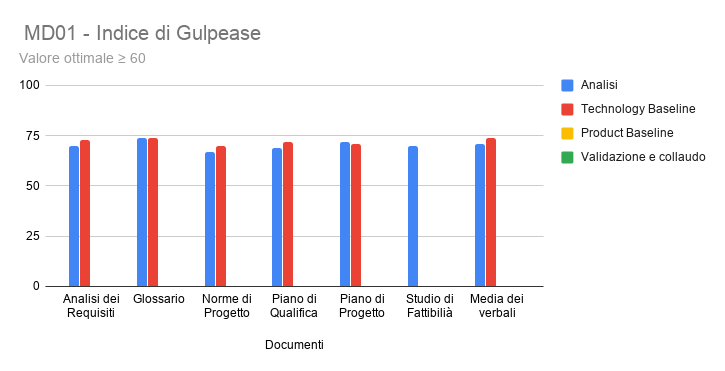
\includegraphics[scale=0.5]{./img/MD01_gulpease.png}
\caption{Grafico relativo ai dati di MD01 - Indice di Gulpease}
\end{figure}

\paragraph{Esiti Indice Fog} \mbox{} \\
\begin{longtable}{c c c c c}
\rowcolor{white}\caption{Tabella Indice Fog} \\
		\rowcolor{redafk}
\textcolor{white}{\textbf{Attività}} &
\textcolor{white}{\textbf{An}} &
\textcolor{white}{\textbf{TB}} &
\textcolor{white}{\textbf{PB}}&
\textcolor{white}{\textbf{VC}}  \\
		\endfirsthead
		\rowcolor{white}\caption[]{(continua)} \\
		\rowcolor{redafk}
\textcolor{white}{\textbf{Attività}} &
\textcolor{white}{\textbf{An}} &
\textcolor{white}{\textbf{TB}} &
\textcolor{white}{\textbf{PB}}&
\textcolor{white}{\textbf{VC}}  \\
		\endhead
Analisi dei Requisiti & 18 & 17 & - & - \\
Glossario & 15 & 15 & - & - \\
Norme di Progetto & 20 & 18 & - & - \\
Piano di Qualifica & 18 & 20 & - & - \\
Piano di Progetto & 20 & 20 & - & - \\
Studio di Fattibilità & 14 & - & & \\
Media dei Verbali & 8 & 6 & - & - \\
\end{longtable}

\begin{figure}[H]
\centering
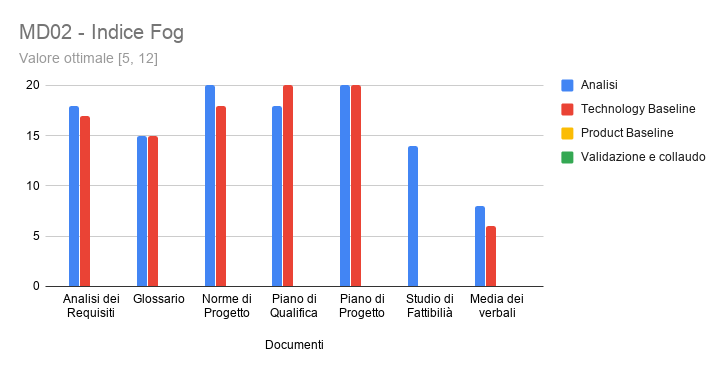
\includegraphics[scale=0.5]{./img/MD02_fog.png}
\caption{Grafico relativo ai dati di MD02 - Indice Fog}
\end{figure}

\subsubsection{Analisi dei processi}
\paragraph{Esiti MP01 - Schedule Variance} \mbox{} \\
\begin{longtable}{c c c c c c}
\rowcolor{white}\caption{Esiti verifica dei processi con Schedule Variance nel periodo di Analisi} \\
		\rowcolor{redafk}
\textcolor{white}{\textbf{Attività}} &
\textcolor{white}{\textbf{An}} &
\textcolor{white}{\textbf{TB}} &
\textcolor{white}{\textbf{PB}} &
\textcolor{white}{\textbf{VC}} &
\textcolor{white}{\textbf{Riscontro}} \\
		\endfirsthead
		\rowcolor{white}\caption[]{(continua)} \\
		\rowcolor{redafk}
\textcolor{white}{\textbf{Attività}} &
\textcolor{white}{\textbf{An}} &
\textcolor{white}{\textbf{TB}} &
\textcolor{white}{\textbf{PB}} &
\textcolor{white}{\textbf{VC}} &
\textcolor{white}{\textbf{Riscontro}} \\
		\endhead
Stestura Analisi dei Requisiti & 
1 &
- &
- &
- &
Accettabile \\
Stestura Glossario & 
0 &
- &
- &
- &
Ottimale \\
Stestura Norme di Progetto & 
0 &
- &
- &
- &
Ottimale \\
Stestura Piano di Qualifica & 
1 &
- &
- &
- &
Accettabile \\
Stestura Piano di Progetto & 
1 &
- &
- &
- &
Accettabile \\
Stestura Studio di Fattibilià & 
0 &
- &
- &
- &
Ottimale \\
\end{longtable}

\begin{figure}[H]
\centering
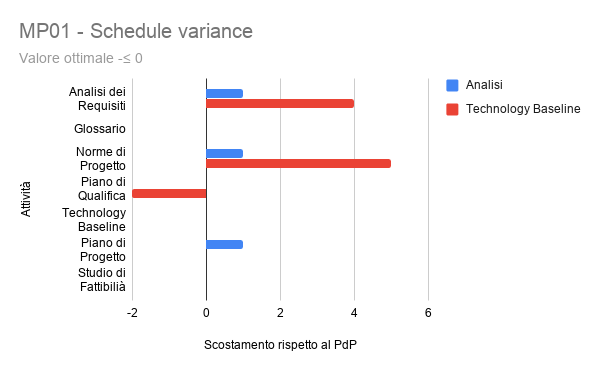
\includegraphics[scale=0.5]{./img/MP01_schedule_variance.png}
\caption{Grafico relativo ai dati di MP01 - Schedule Variance}
\end{figure}

\paragraph{Esiti MP02 - Budget Variance} \mbox{} \\ \mbox{} \\
\begin{longtable}{c c c c c}
\rowcolor{white}\caption{Esiti Budget Variance} \\
		\rowcolor{redafk}
\textcolor{white}{\textbf{An}} &
\textcolor{white}{\textbf{TB}} &
\textcolor{white}{\textbf{PB}} &
\textcolor{white}{\textbf{VC}} &
\textcolor{white}{\textbf{Riscontro}} \\
-8,66$\%$ &
-1,19$\%$ &
- &
- &
Accettabile \\
\end{longtable}

\begin{figure}[H]
\centering
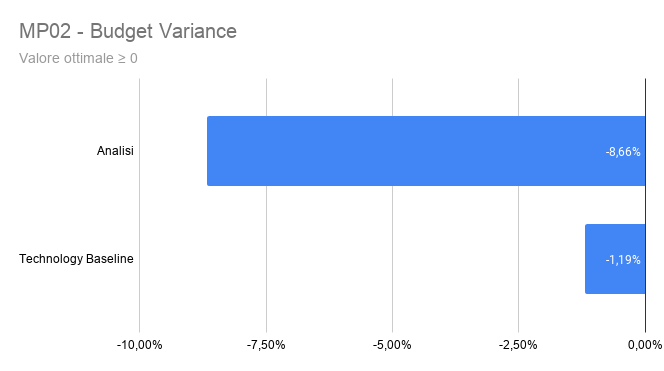
\includegraphics[scale=0.5]{./img/MP02_budget_variance.png}
\caption{Grafico relativo ai dati di MP02 - Budget Variance}
\end{figure}

\paragraph{Esiti MP03 - Produttività} \mbox{} \\ \mbox{} \\
\begin{longtable}{c c c c c c}
\rowcolor{white}\caption{Esiti della Produttività} \\
		\rowcolor{redafk}
\textcolor{white}{\textbf{Membro}} &
\textcolor{white}{\textbf{An}} &
\textcolor{white}{\textbf{TB}} &
\textcolor{white}{\textbf{PB}} &
\textcolor{white}{\textbf{VC}} &
\textcolor{white}{\textbf{Riscontro}} \\
		\endfirsthead
		\rowcolor{white}\caption[]{(continua)} \\
		\rowcolor{redafk}
		\textcolor{white}{\textbf{Membro}} &
\textcolor{white}{\textbf{An}} &
\textcolor{white}{\textbf{TB}} &
\textcolor{white}{\textbf{PB}} &
\textcolor{white}{\textbf{VC}} &
\textcolor{white}{\textbf{Riscontro}} \\
		\endhead
Simone Federico Bergamin & 0 & - & - & - & ----- \\
Alessandro Canesso & 0 & - & - & - & ----- \\
Victor Dutca & 0 & - & - & - & ----- \\
Fouad Farid & 0 & - & - & - & ----- \\
Simone Meneghin & 0 & - & - & - & ----- \\
Olivier Utshudi & 0 & - & - & - & ----- \\
Davide Zillio & 0 & - & - & - & ----- \\
\end{longtable}